% Options for packages loaded elsewhere
\PassOptionsToPackage{unicode}{hyperref}
\PassOptionsToPackage{hyphens}{url}
%
\documentclass[
  english,
  man,floatsintext]{apa6}
\usepackage{lmodern}
\usepackage{amssymb,amsmath}
\usepackage{ifxetex,ifluatex}
\ifnum 0\ifxetex 1\fi\ifluatex 1\fi=0 % if pdftex
  \usepackage[T1]{fontenc}
  \usepackage[utf8]{inputenc}
  \usepackage{textcomp} % provide euro and other symbols
\else % if luatex or xetex
  \usepackage{unicode-math}
  \defaultfontfeatures{Scale=MatchLowercase}
  \defaultfontfeatures[\rmfamily]{Ligatures=TeX,Scale=1}
\fi
% Use upquote if available, for straight quotes in verbatim environments
\IfFileExists{upquote.sty}{\usepackage{upquote}}{}
\IfFileExists{microtype.sty}{% use microtype if available
  \usepackage[]{microtype}
  \UseMicrotypeSet[protrusion]{basicmath} % disable protrusion for tt fonts
}{}
\makeatletter
\@ifundefined{KOMAClassName}{% if non-KOMA class
  \IfFileExists{parskip.sty}{%
    \usepackage{parskip}
  }{% else
    \setlength{\parindent}{0pt}
    \setlength{\parskip}{6pt plus 2pt minus 1pt}}
}{% if KOMA class
  \KOMAoptions{parskip=half}}
\makeatother
\usepackage{xcolor}
\IfFileExists{xurl.sty}{\usepackage{xurl}}{} % add URL line breaks if available
\IfFileExists{bookmark.sty}{\usepackage{bookmark}}{\usepackage{hyperref}}
\hypersetup{
  pdftitle={The Sound of Teaching Music: Expert Pianists' Performance Modulations for Novices},
  pdflang={en-EN},
  pdfkeywords={teaching, expertise, skill transmission, artistic expression, music},
  hidelinks,
  pdfcreator={LaTeX via pandoc}}
\urlstyle{same} % disable monospaced font for URLs
\usepackage{graphicx}
\makeatletter
\def\maxwidth{\ifdim\Gin@nat@width>\linewidth\linewidth\else\Gin@nat@width\fi}
\def\maxheight{\ifdim\Gin@nat@height>\textheight\textheight\else\Gin@nat@height\fi}
\makeatother
% Scale images if necessary, so that they will not overflow the page
% margins by default, and it is still possible to overwrite the defaults
% using explicit options in \includegraphics[width, height, ...]{}
\setkeys{Gin}{width=\maxwidth,height=\maxheight,keepaspectratio}
% Set default figure placement to htbp
\makeatletter
\def\fps@figure{htbp}
\makeatother
\setlength{\emergencystretch}{3em} % prevent overfull lines
\providecommand{\tightlist}{%
  \setlength{\itemsep}{0pt}\setlength{\parskip}{0pt}}
\setcounter{secnumdepth}{-\maxdimen} % remove section numbering
% Make \paragraph and \subparagraph free-standing
\ifx\paragraph\undefined\else
  \let\oldparagraph\paragraph
  \renewcommand{\paragraph}[1]{\oldparagraph{#1}\mbox{}}
\fi
\ifx\subparagraph\undefined\else
  \let\oldsubparagraph\subparagraph
  \renewcommand{\subparagraph}[1]{\oldsubparagraph{#1}\mbox{}}
\fi
% Manuscript styling
\usepackage{upgreek}
\captionsetup{font=singlespacing,justification=justified}

% Table formatting
\usepackage{longtable}
\usepackage{lscape}
% \usepackage[counterclockwise]{rotating}   % Landscape page setup for large tables
\usepackage{multirow}		% Table styling
\usepackage{tabularx}		% Control Column width
\usepackage[flushleft]{threeparttable}	% Allows for three part tables with a specified notes section
\usepackage{threeparttablex}            % Lets threeparttable work with longtable

% Create new environments so endfloat can handle them
% \newenvironment{ltable}
%   {\begin{landscape}\begin{center}\begin{threeparttable}}
%   {\end{threeparttable}\end{center}\end{landscape}}
\newenvironment{lltable}{\begin{landscape}\begin{center}\begin{ThreePartTable}}{\end{ThreePartTable}\end{center}\end{landscape}}

% Enables adjusting longtable caption width to table width
% Solution found at http://golatex.de/longtable-mit-caption-so-breit-wie-die-tabelle-t15767.html
\makeatletter
\newcommand\LastLTentrywidth{1em}
\newlength\longtablewidth
\setlength{\longtablewidth}{1in}
\newcommand{\getlongtablewidth}{\begingroup \ifcsname LT@\roman{LT@tables}\endcsname \global\longtablewidth=0pt \renewcommand{\LT@entry}[2]{\global\advance\longtablewidth by ##2\relax\gdef\LastLTentrywidth{##2}}\@nameuse{LT@\roman{LT@tables}} \fi \endgroup}

% \setlength{\parindent}{0.5in}
% \setlength{\parskip}{0pt plus 0pt minus 0pt}

% \usepackage{etoolbox}
\makeatletter
\patchcmd{\HyOrg@maketitle}
  {\section{\normalfont\normalsize\abstractname}}
  {\section*{\normalfont\normalsize\abstractname}}
  {}{\typeout{Failed to patch abstract.}}
\makeatother
\shorttitle{The Sound of Teaching Music}
\author{Atsuko Tominaga\textsuperscript{1}, Günther Knoblich\textsuperscript{1}, \& Natalie Sebanz\textsuperscript{1}}
\affiliation{
\vspace{0.5cm}
\textsuperscript{1} Department of Cognitive Science, Central European University}
\authornote{

Correspondence concerning this article should be addressed to Atsuko Tominaga, Quellenstraße 51, 1100 Vienna, Austria. E-mail: Tominaga\_Atsuko@phd.ceu.edu}
\keywords{teaching, expertise, skill transmission, artistic expression, music\newline\indent Word count: X}
\usepackage{lineno}

\linenumbers
\usepackage{csquotes}
\ifxetex
  % Load polyglossia as late as possible: uses bidi with RTL langages (e.g. Hebrew, Arabic)
  \usepackage{polyglossia}
  \setmainlanguage[]{english}
\else
  \usepackage[shorthands=off,main=english]{babel}
\fi
\ifluatex
  \usepackage{selnolig}  % disable illegal ligatures
\fi
\newlength{\cslhangindent}
\setlength{\cslhangindent}{1.5em}
\newenvironment{cslreferences}%
  {}%
  {\par}

\title{The Sound of Teaching Music: Expert Pianists' Performance Modulations for Novices}

\date{}

\abstract{
One or two sentences providing a \textbf{basic introduction} to the field, comprehensible to a scientist in any discipline.

Two to three sentences of \textbf{more detailed background}, comprehensible to scientists in related disciplines.

One sentence clearly stating the \textbf{general problem} being addressed by this particular study.

One sentence summarizing the main result (with the words ``\textbf{here we show}'' or their equivalent).

Two or three sentences explaining what the \textbf{main result} reveals in direct comparison to what was thought to be the case previously, or how the main result adds to previous knowledge.

One or two sentences to put the results into a more \textbf{general context}.

Two or three sentences to provide a \textbf{broader perspective}, readily comprehensible to a scientist in any discipline.
}

\begin{document}
\maketitle

\hypertarget{introduction}{%
\section{1. Introduction}\label{introduction}}

\hypertarget{experiment-1}{%
\section{2. Experiment 1}\label{experiment-1}}

\hypertarget{method}{%
\subsection{2.1. Method}\label{method}}

\hypertarget{participants}{%
\subsubsection{2.1.1. Participants}\label{participants}}

We recruited 36 piano experts who played the piano for at least the past 10 years or were studying piano performance at a music school at the time of recruitment. For data analysis, we excluded 5 participants due to an experimental error (3), an overall deviated tempo (2). Thirty-one participants (15 female) were included in data analysis. They had 12.45 years of practice on average (\emph{SD} = 5.66). All participants gave their informed consent before the experiment started and received vouchers for their participation. The study was approved by the United Ethical REview Committee for Research in Psychology (EPKEB) in Hungary.

\hypertarget{apparatus-and-stimuli}{%
\subsubsection{2.1.2. Apparatus and stimuli}\label{apparatus-and-stimuli}}

A weighted Yamaha MIDI digital piano was used to record participants' performance via Max/MSP on a MacBook Pro with MacOS X Mojave 10.14.3. The laptop and piano were connected to a high-fidelity soundcard (Focusrite Scarlett 6i6) to deliver a metronome and piano sound. All auditory feedback was given to participants through headphones (Audio-Technica ATH-M50X). Sheet music was displayed on a computer monitor in front of the participants. The pitch, onset and offset time of each note, and key velocity profiles were obtained from MIDI data using Max/MSP patchers.

One musical excerpt was used as a stimulus. The excerpt was taken from ``A Dozen a Day - Play with Ease in Many Keys" by Edna-Mae Brunam and modified for the experiment. It consisted of a 6-measure isochronous melody noted in 4/4 meter. The stimulus was composed in C major to be played with the right hand only. Non-expressive sheet music (i.e., sheet music without musical expression; see \emph{Figure \ref{fig:stimuli}, A}) was used for the purpose of practice. Expressive notations were added to the non-expressive sheet music for the experiment. They referred to either articulation or dynamics (\emph{Figure \ref{fig:stimuli}, B-C}). Articulation was notated as either legato or staccato. Legato indicates that musical notes are to be connected and should sound smooth. Staccato requires producing musical notes with shortened duration, keeping them separate from each other. Dynamics was notated in terms of forte and piano. Forte indicates that musical notes should be played loudly whereas piano indicates that musical notes should be played softly. The notation did not include any indication of fingering (i.e., the positioning of the fingers when playing the piano) because the piece was simple and pilot testing had shown that specifying fingering was not required.

\hypertarget{procedure}{%
\subsubsection{2.1.3. Procedure}\label{procedure}}

In order to ensure that participants had sufficient motor skills to perform the piece, we asked them to practise the piece with the non-expressive sheet music (\emph{Figure \ref{fig:stimuli}, A}). Once they could perform the piece without pitch errors twice consecutively, the experiment started.

First, participants were allocated to either the teaching or performing condition and asked to practise the excerpt the excerpt with notated expressions of either articulation or dynamics (\emph{Figure \ref{fig:stimuli}, B-C}). As soon as they had produced the excerpt with notated expressions without pitch errors twice consecutively, the test trials began.

In the teaching condition, participants were instructed to play the excerpt of music as if they were teaching it to students. It was mentioned that the students already knew the sequence of the tones and that they were trying to learn how to perform the piece with notated expressions by listening to the participant's performance. In the performing condition, participants were asked to play the excerpt of music as if they were performing it to an audience. Participants played the piece 8 times per expressive technique per condition, so there were 32 trials in total (2 conditions x 2 expressive techniques x 8 trials). The order of the conditions was counterbalanced across participants. The order of the expressive techniques within each condition was also counterbalanced across participants. A leading metronome (80 beats per minute, 8 beats) indicated the target tempo before each trial.

At the end of the experiment, participants filled in a questionnaire asking about their demographic information and experience in piano performance/teaching.

\hypertarget{design-and-data-analysis}{%
\subsubsection{2.1.4. Design and data analysis}\label{design-and-data-analysis}}

The experiment had two factors; Condition (teaching vs.~performing) and Expressive Technique (articulation vs.~dynamics). Additionally, the factor Subcomponent was used when analysing data for each subcomponent for each technique separately (i.e., LS; legato vs.~staccato, FP; forte vs.~piano).

Three dependent variables were computed for data analysis. Interonset intervals (IOIs) are the intervals between onsets of adjacent notes and provide a tempo of tempo. Key-overlap time (KOT) is the difference between the offset time of the current tone (i.e., key release time) and the onset time of the ensuing tone and measures the smoothness of musical sequences (CITE). A positive value indicates smooth legato styles due to overlap between the current and ensuing tone whereas a negative value indicates sharp staccato styles due to separation between the current and ensuing tone. Tone intensity is assessed by key velocity (KV) and measures the loudness of a musical note. The value of KV in MIDI varies between 0 (minimum) and 127 (maximum).

Pitch errors were identified by comparing the participants' performance with the sheet music. (TBC)

\begin{figure}
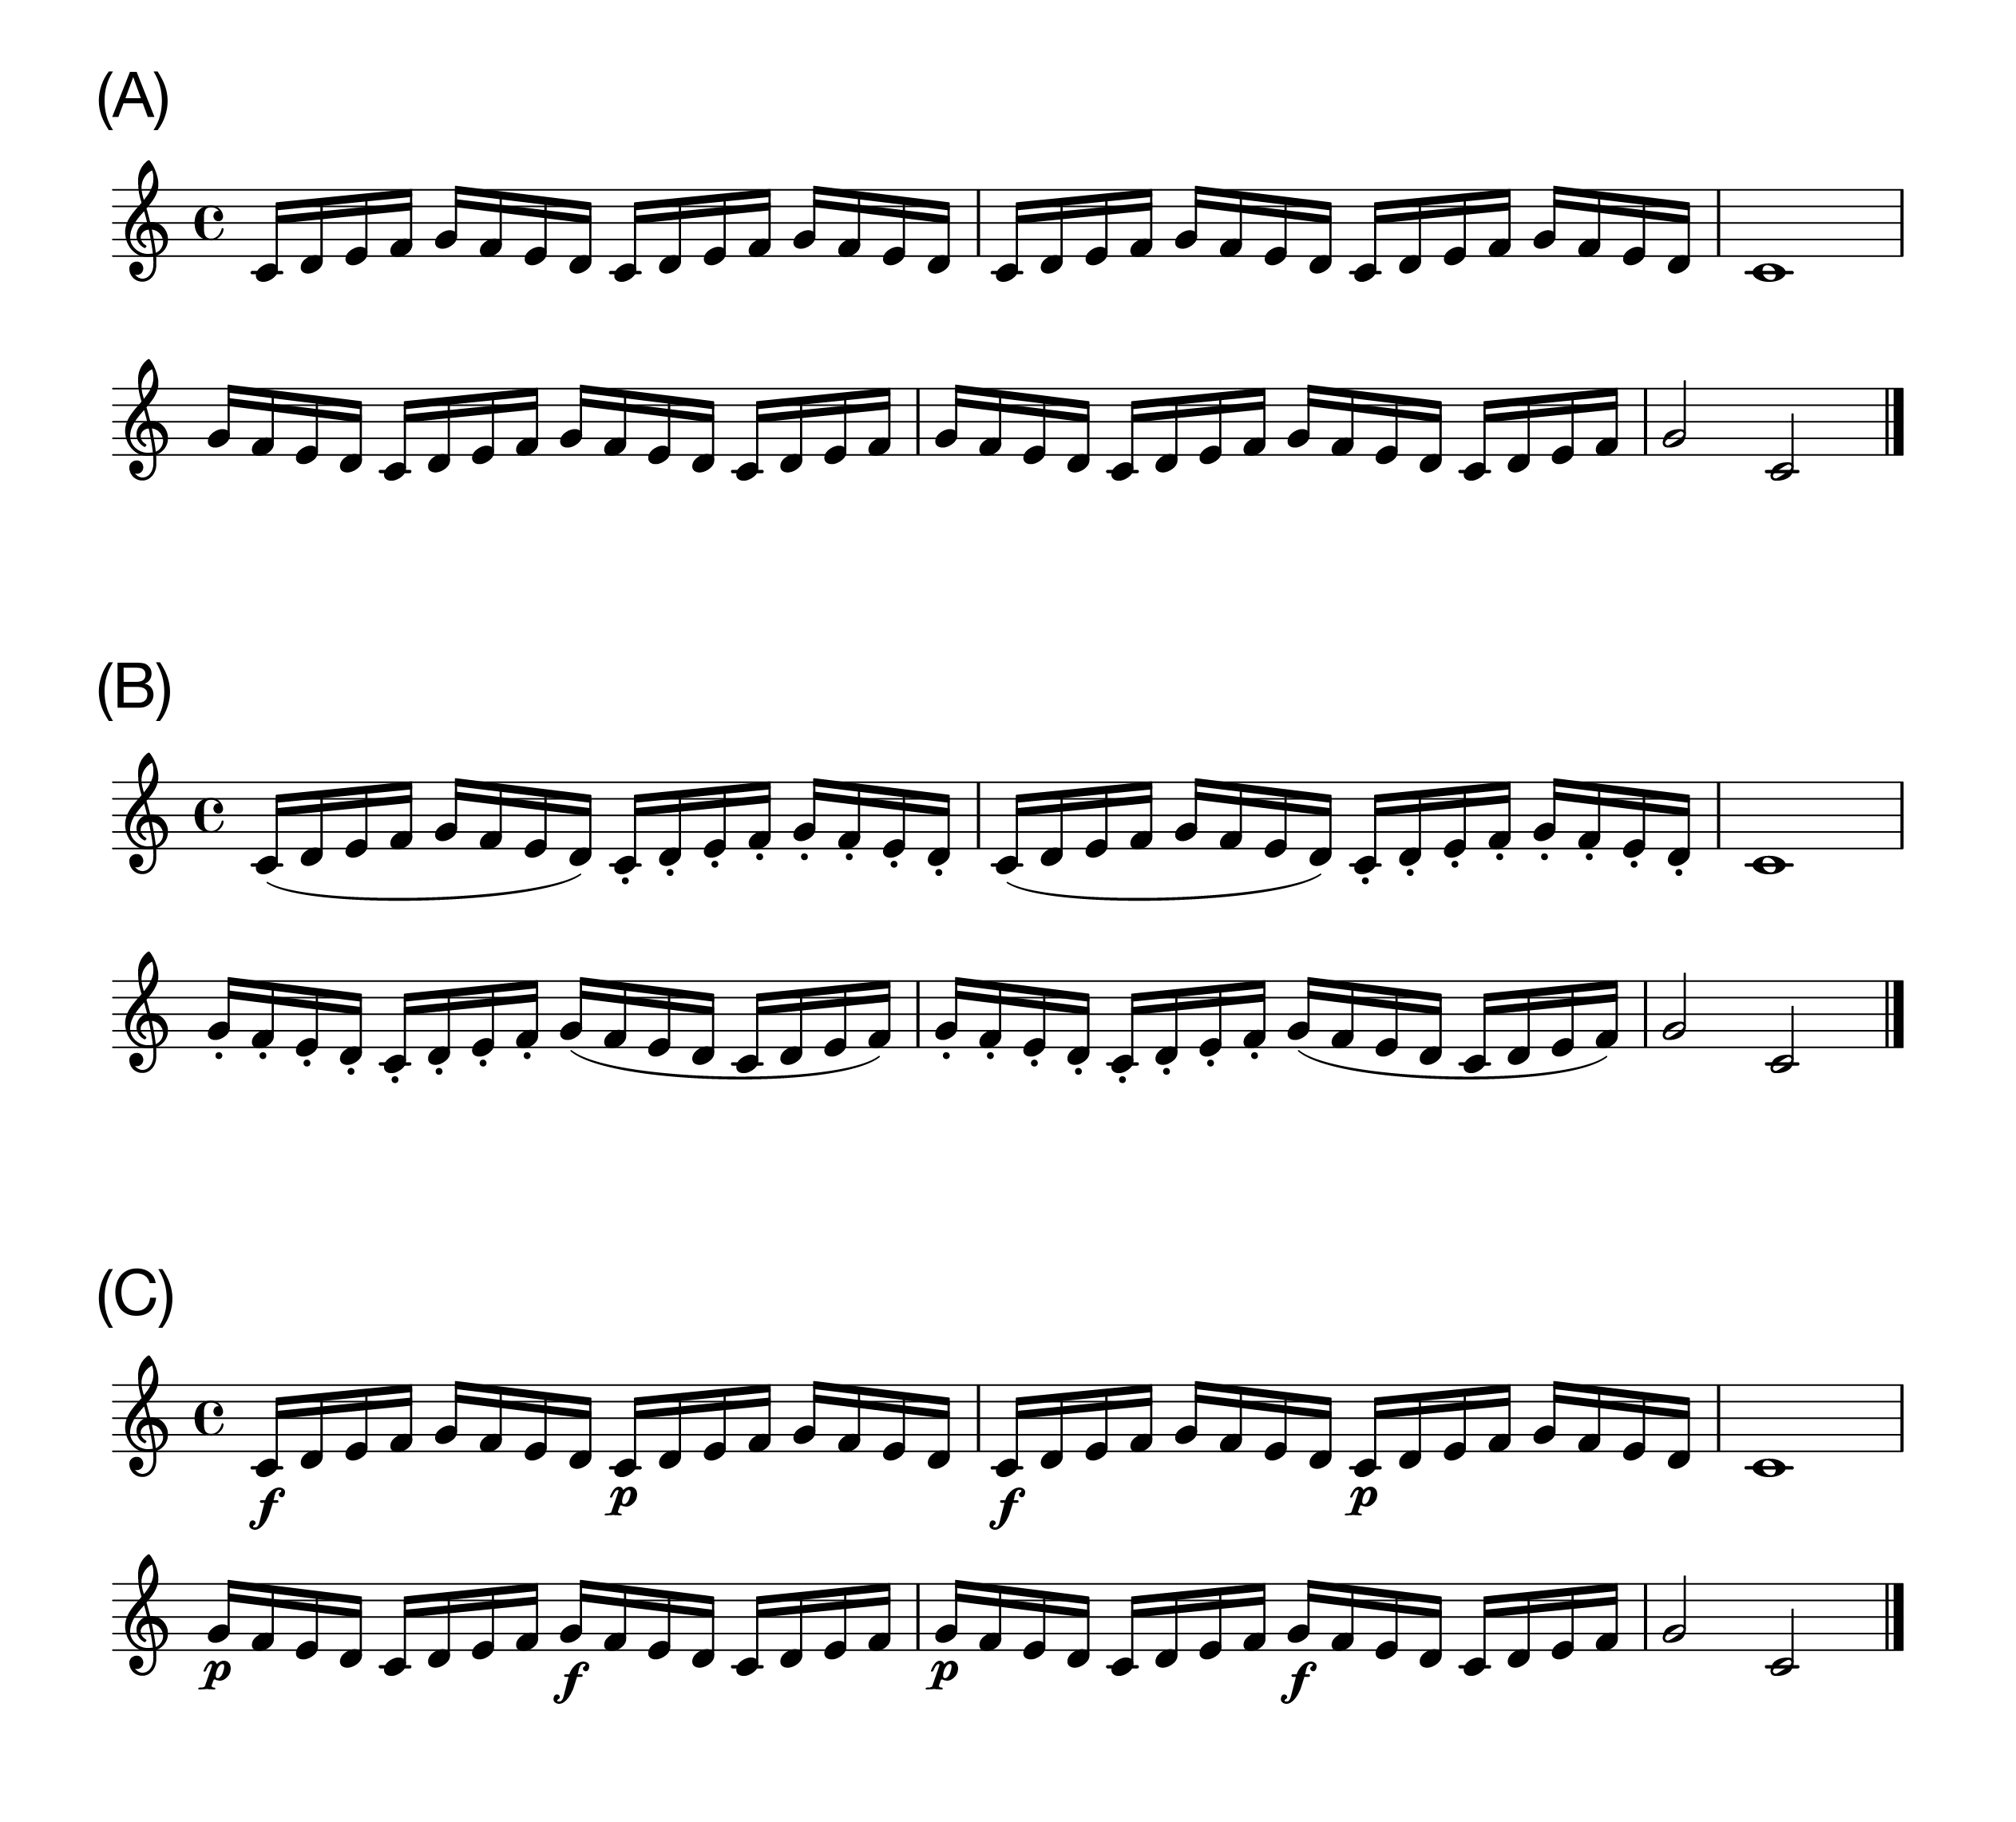
\includegraphics[width=1\linewidth]{manuscript_files/figure-latex/stim-1-1} \caption{\label{fig:stimuli}(A)Non-expressive sheet music. (B)Articulation. The curved line (slur) indicates legato and the dots indicate staccato. (C)Dynamics. The symbol `f' denotes forte and the symbol `p' denotes piano. For data analysis, only the 16th notes were included.}\label{fig:stim-1}
\end{figure}

\hypertarget{results-articulation}{%
\subsection{2.2. Results (Articulation)}\label{results-articulation}}

\hypertarget{interonset-intervals-iois}{%
\subsubsection{2.2.1. Interonset Intervals (IOIs)}\label{interonset-intervals-iois}}

\hypertarget{key-overlap-time-kot}{%
\subsubsection{2.2.2. Key-Overlap Time (KOT)}\label{key-overlap-time-kot}}

\hypertarget{key-velocity-kv}{%
\subsubsection{2.2.3. Key Velocity (KV)}\label{key-velocity-kv}}

\hypertarget{kv-transition-points}{%
\subsubsection{2.2.4. KV Transition Points}\label{kv-transition-points}}

\hypertarget{results-dynamics}{%
\subsection{2.3. Results (Dynamics)}\label{results-dynamics}}

\hypertarget{interonset-intervals-iois-1}{%
\subsubsection{2.3.1. Interonset Intervals (IOIs)}\label{interonset-intervals-iois-1}}

\hypertarget{key-velocity-kv-1}{%
\subsubsection{2.3.2. Key Velocity (KV)}\label{key-velocity-kv-1}}

\hypertarget{kv-transition-points-1}{%
\subsubsection{2.3.3. KV Transition Points}\label{kv-transition-points-1}}

\hypertarget{key-overlap-time-kot-1}{%
\subsubsection{2.3.4. Key-Overlap Time (KOT)}\label{key-overlap-time-kot-1}}

\hypertarget{discussion}{%
\subsection{2.4. Discussion}\label{discussion}}

\newpage

\hypertarget{experiment-2}{%
\section{3. Experiment 2}\label{experiment-2}}

\hypertarget{method-1}{%
\subsection{3.1. Method}\label{method-1}}

\hypertarget{participants-1}{%
\subsubsection{3.1.1. Participants}\label{participants-1}}

We recruited 21 piano experts who already had a degree in (above bachelor or equivalent) in piano performance/teaching or were studying piano performance at a music school at the time of recruitment. One participant was excluded due to insufficient motor skills. Twenty participants (9 female) were included in data analysis. They had 15.65 years of practice on average (\emph{SD} = 5.67).

\hypertarget{apparatus-and-stimuli-1}{%
\subsubsection{3.1.2. Apparatus and stimuli}\label{apparatus-and-stimuli-1}}

The same apparatus as Experiment 1 was used. We selected Clementi's Sonatina Op.36 (No.3) in C major as a stimulus because it contained our targeted expression (i.e., articulation, dynamics) and relatively simple in terms of motor skills. The first 12 measures of the original piece and modified it so that it had the most equal number of data points for each dependent variable (see details in \emph{\protect\hyperlink{analysis-2}{Data analysis}}). The stimulus consisted of a 12-measure isochronous melody notated in 4/4 meter. Only the right hand was used to play. Non-expressive sheet was used for the purpose of practice (\emph{Figure \ref{fig:stimuli-2}, A}). Expressive notations were added to the non-expressive sheet music for the experiment (\emph{Figure \ref{fig:stimuli-2}, B-C}). These excerpts were confirmed to be musically natural by a doctoral student in piano performance at Liszt Ferenc Academy of Music in Hungary. The fingering was also assigned and confirmed by the same doctoral student.

\hypertarget{procedure-1}{%
\subsubsection{3.1.3. Procedure}\label{procedure-1}}

\hypertarget{design-and-data-analysis-1}{%
\subsubsection{3.1.4. Design and data analysis}\label{design-and-data-analysis-1}}

\begin{figure}
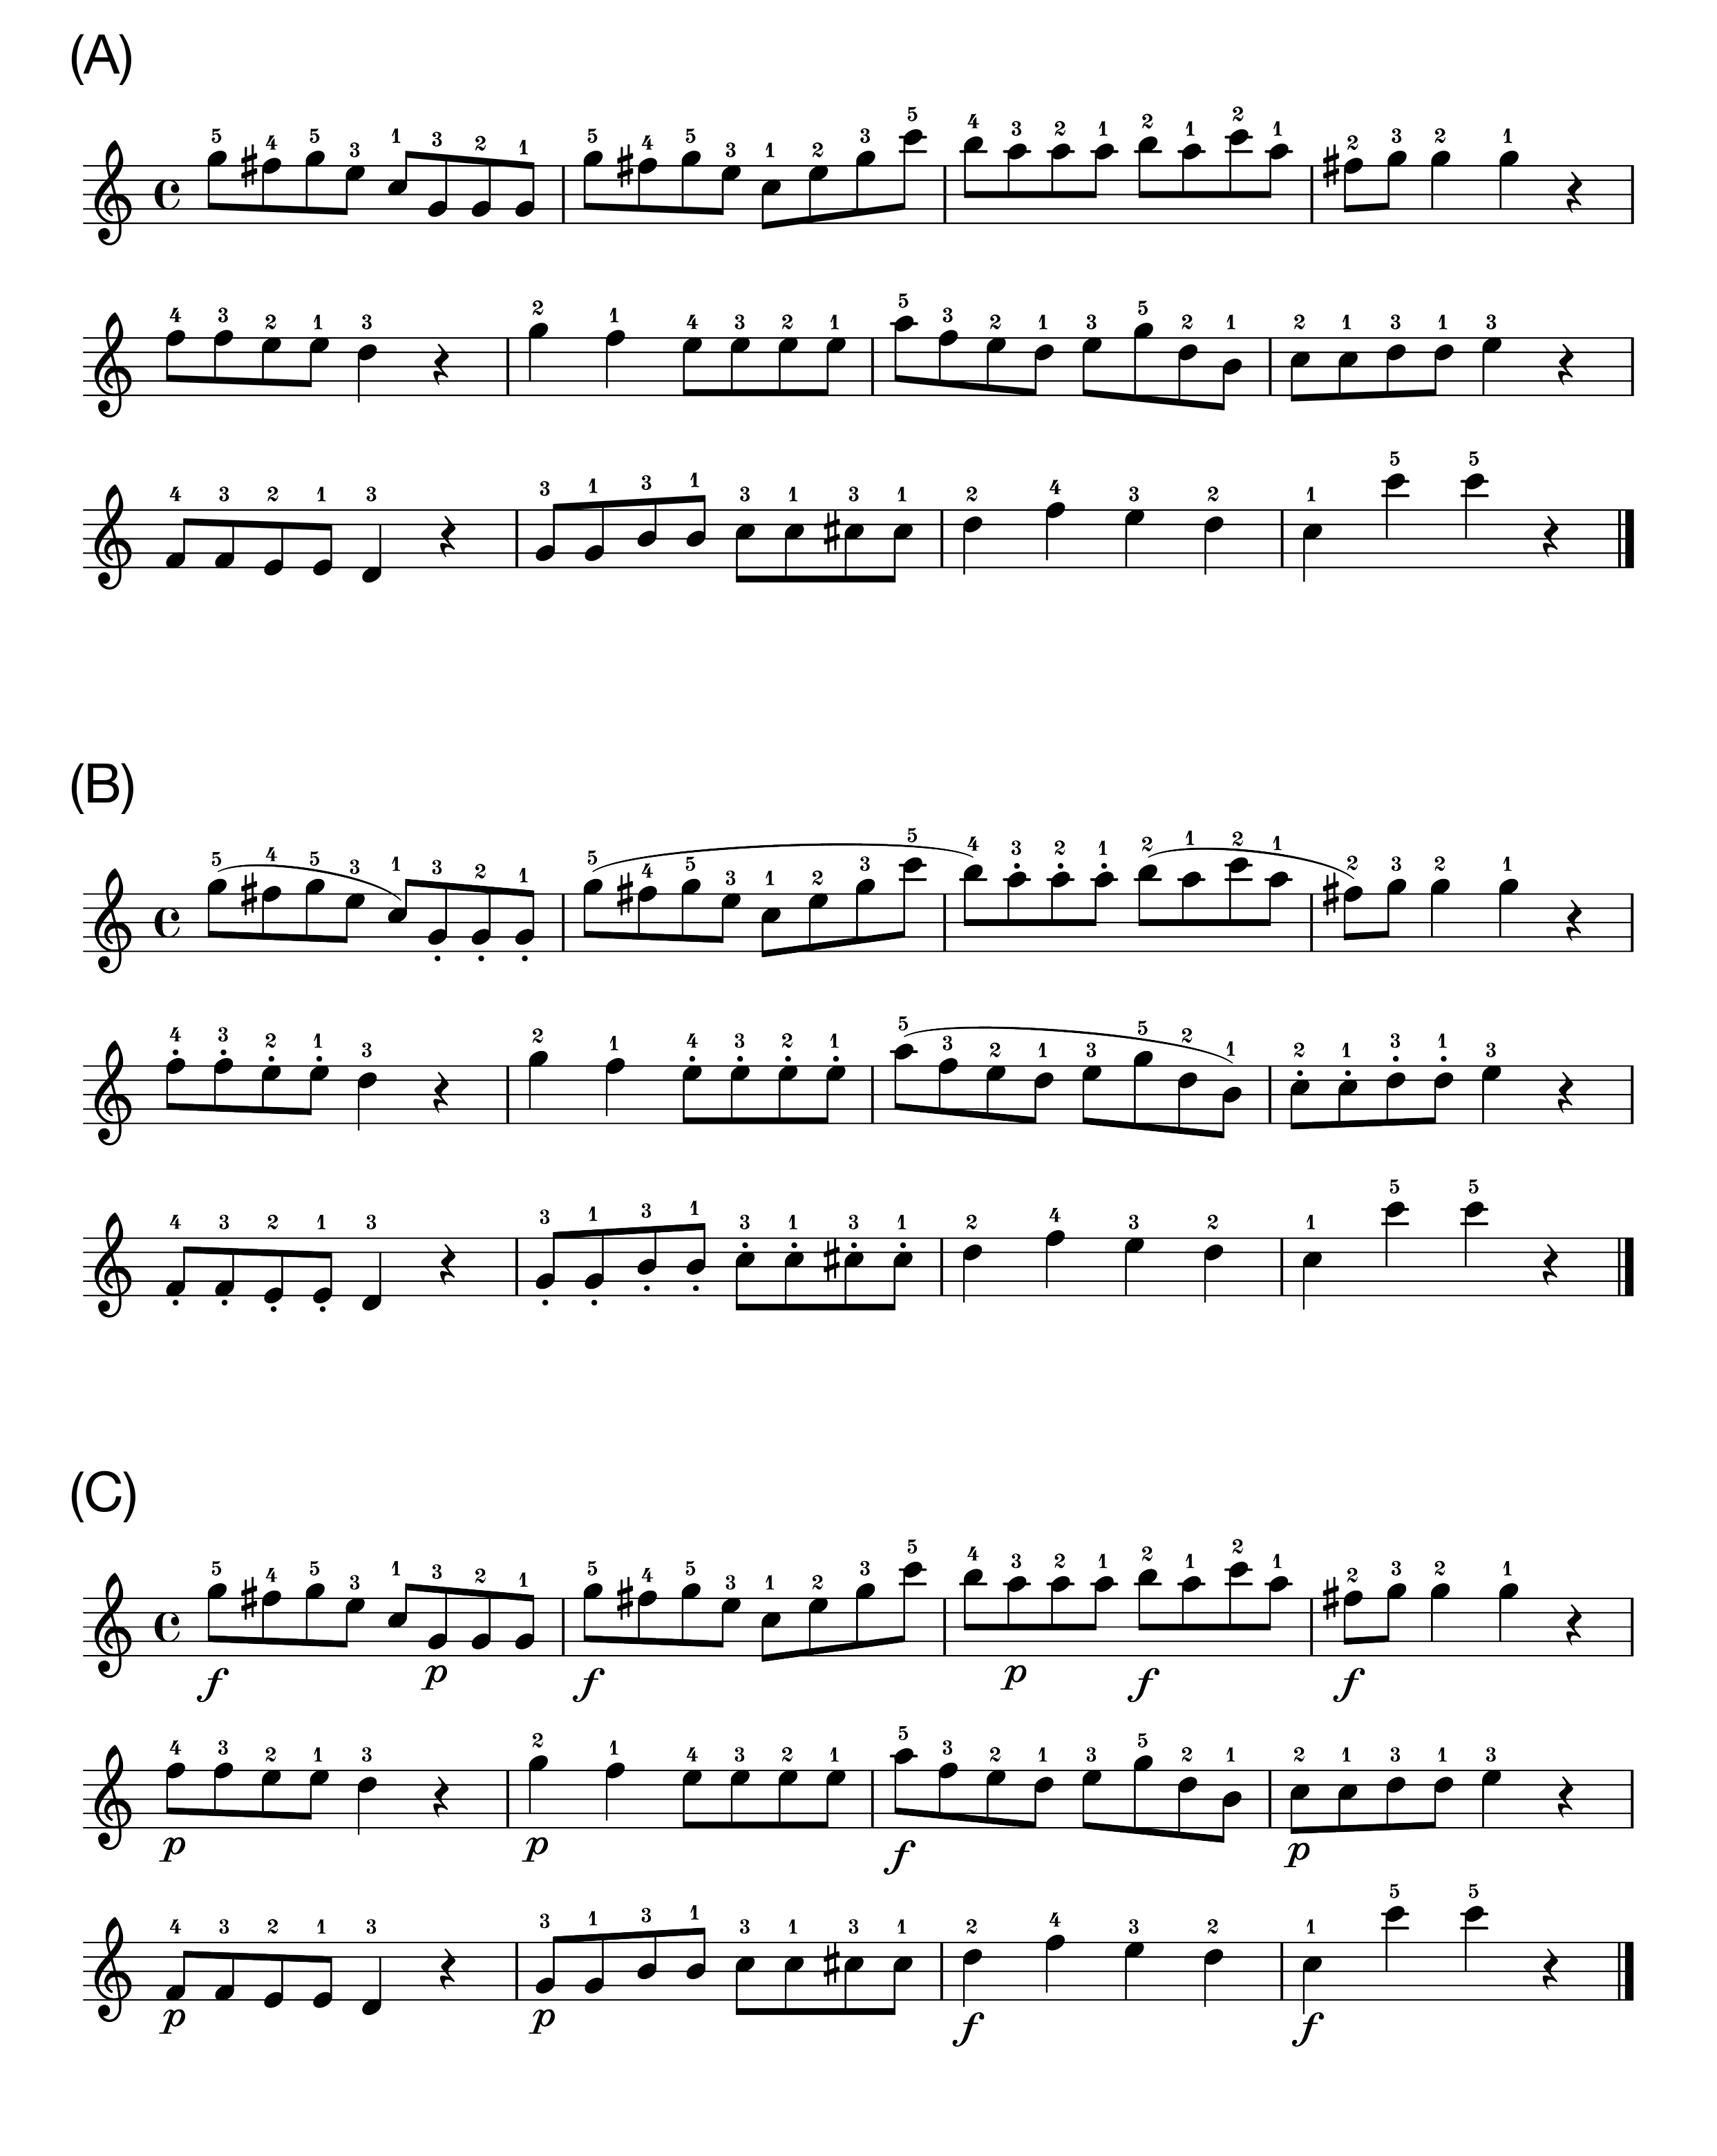
\includegraphics[width=1\linewidth]{manuscript_files/figure-latex/stim-2-1} \caption{\label{fig:stimuli-2}(A)Non-expressive sheet music. (B)Articulation. The curved line (slur) indicates legato and the dots indicate staccato. (C)Dynamics. The symbol `f' denotes forte and the symbol `p' denotes piano. For data analysis, only the 16th notes were included.}\label{fig:stim-2}
\end{figure}

\hypertarget{results-articulation-1}{%
\subsection{3.2. Results (Articulation)}\label{results-articulation-1}}

\hypertarget{interonset-intervals-iois-2}{%
\subsubsection{3.2.1. Interonset Intervals (IOIs)}\label{interonset-intervals-iois-2}}

\hypertarget{key-overlap-time-kot-2}{%
\subsubsection{3.2.2. Key-Overlap Time (KOT)}\label{key-overlap-time-kot-2}}

\hypertarget{key-velocity-kv-2}{%
\subsubsection{3.2.3. Key Velocity (KV)}\label{key-velocity-kv-2}}

\hypertarget{kv-transition-points-2}{%
\subsubsection{3.2.4. KV Transition Points}\label{kv-transition-points-2}}

\hypertarget{results-dynamics-1}{%
\subsection{3.3. Results (Dynamics)}\label{results-dynamics-1}}

\hypertarget{interonset-intervals-iois-3}{%
\subsubsection{3.3.1. Interonset Intervals (IOIs)}\label{interonset-intervals-iois-3}}

\hypertarget{key-velocity-kv-3}{%
\subsubsection{3.3.2. Key Velocity (KV)}\label{key-velocity-kv-3}}

\hypertarget{kv-transition-points-3}{%
\subsubsection{3.3.3. KV Transition Points}\label{kv-transition-points-3}}

\hypertarget{key-overlap-time-kot-3}{%
\subsubsection{3.3.4. Key-Overlap Time (KOT)}\label{key-overlap-time-kot-3}}

\hypertarget{discussion-1}{%
\subsection{3.4. Discussion}\label{discussion-1}}

\newpage

\hypertarget{general-discussion}{%
\section{4. General Discussion}\label{general-discussion}}

\hypertarget{acknowledgements}{%
\section{Acknowledgements}\label{acknowledgements}}

We thank Dávid Csűrös for his help with data collection. This research was supported by the European Research Council under the European Union's Seventh Framework Program (FP7/2007-2013)/ERC (European Research Council) grant agreement no. 609819, SOMICS, and by ERC grant agreement no. 616072, JAXPERTISE.

\hypertarget{declarations-of-interest}{%
\section{Declarations of interest}\label{declarations-of-interest}}

All authors have no conflict of interest.

\newpage

\hypertarget{references}{%
\section{References}\label{references}}

\begingroup
\setlength{\parindent}{-0.5in}
\setlength{\leftskip}{0.5in}

\hypertarget{refs}{}
\begin{cslreferences}
\end{cslreferences}

\endgroup
\raggedbottom

\end{document}
